\documentclass[hyperref={pdfpagelabels=false}]{beamer}

\usetheme{Heidelberg}

\usepackage{wrapfig}
\usepackage{lmodern}
\usepackage{natbib}
\usepackage{amsmath,amsfonts,amssymb}
\usepackage{algorithm,algorithmic}
%\floatname{algorithm}{Algorithmus}

%\usepackage{tikz}
%	\usetikzlibrary[topaths,arrows,calc]
\usepackage{wrapfig}
\usepackage{graphicx}
\usepackage{subcaption}


\usepackage[english]{babel}
\usepackage[T1]{fontenc} % Ligaturen, richtige Umlaute im PDF 
\usepackage[utf8]{inputenc}% UTF8-Kodierung für Umlaute usw

\usepackage{hyperref}

\definecolor{darkred}{rgb}{110,1,1}  
\definecolor{maroon}{rgb}{0.5,0,0}  

\newcounter{saveenumi}
\newcommand{\seti}{\setcounter{saveenumi}{\value{enumi}}}
\newcommand{\conti}{\setcounter{enumi}{\value{saveenumi}}}


% zusaetzlich ist das usepackage{beamerthemeshadow} eingebunden 
\usepackage{beamerthemeshadow}

\renewcommand{\thefootnote}{\fnsymbol{footnote}} 

%--------------------------------------------------------------------------%
%--------------------------------------------------------------------------%
\def\vec{\mathop{\rm vec}}								% matrix vectorization
\def\tr{\mathop{\rm tr}}								% matrix trace
\def\argmax{\mathop{\rm argmax}}						% argmax
\def\argmin{\mathop{\rm argmin}}						% argmin
\def\median{\mathop{\rm median}} 						% median
\def\dist{\mathop{\rm dist}} 						    % dist
%--------------------------------------------------------------------------%
%--------------------------------------------------------------------------%
\title[Application of graph matching in Computer Vision]
	{Application of graph matching in Computer Vision}
\subtitle{Master Seminar}
\author[E.~Tikhoncheva] % (optional, for multiple authors)
	{Ekaterina~Tikhoncheva}
\institute[Universities Here and There] % (optional)
	{University of Heidelberg\\
	Faculty of Mathematics and Computer Science \\
	Computer Vision group \\
	at\\
	Heidelberg Collaboratory for Image Processing
}
\date[2015]{November 2015}
%--------------------------------------------------------------------------%
%--------------------------------------------------------------------------%
%--------------------------------------------------------------------------%
\begin{document}
\begin{frame}
\titlepage
\end{frame}
%--------------------------------------------------------------------------%
\begin{frame}
\frametitle{Agenda}
\tableofcontents
\end{frame} 
%--------------------------------------------------------------------------%
%--------------------------------------------------------------------------%
\section{Graph matching} 

\begin{frame}[allowframebreaks]
\frametitle{Attributed undirected graph}

Attributed undirected graph $G=(V,$
\begin{itemize}
\item set of nodes $V=\{v_i\}_{i=1}^{n}$
\end{itemize}
\vspace{2cm}
\begin{figure}[b]
    \centering
    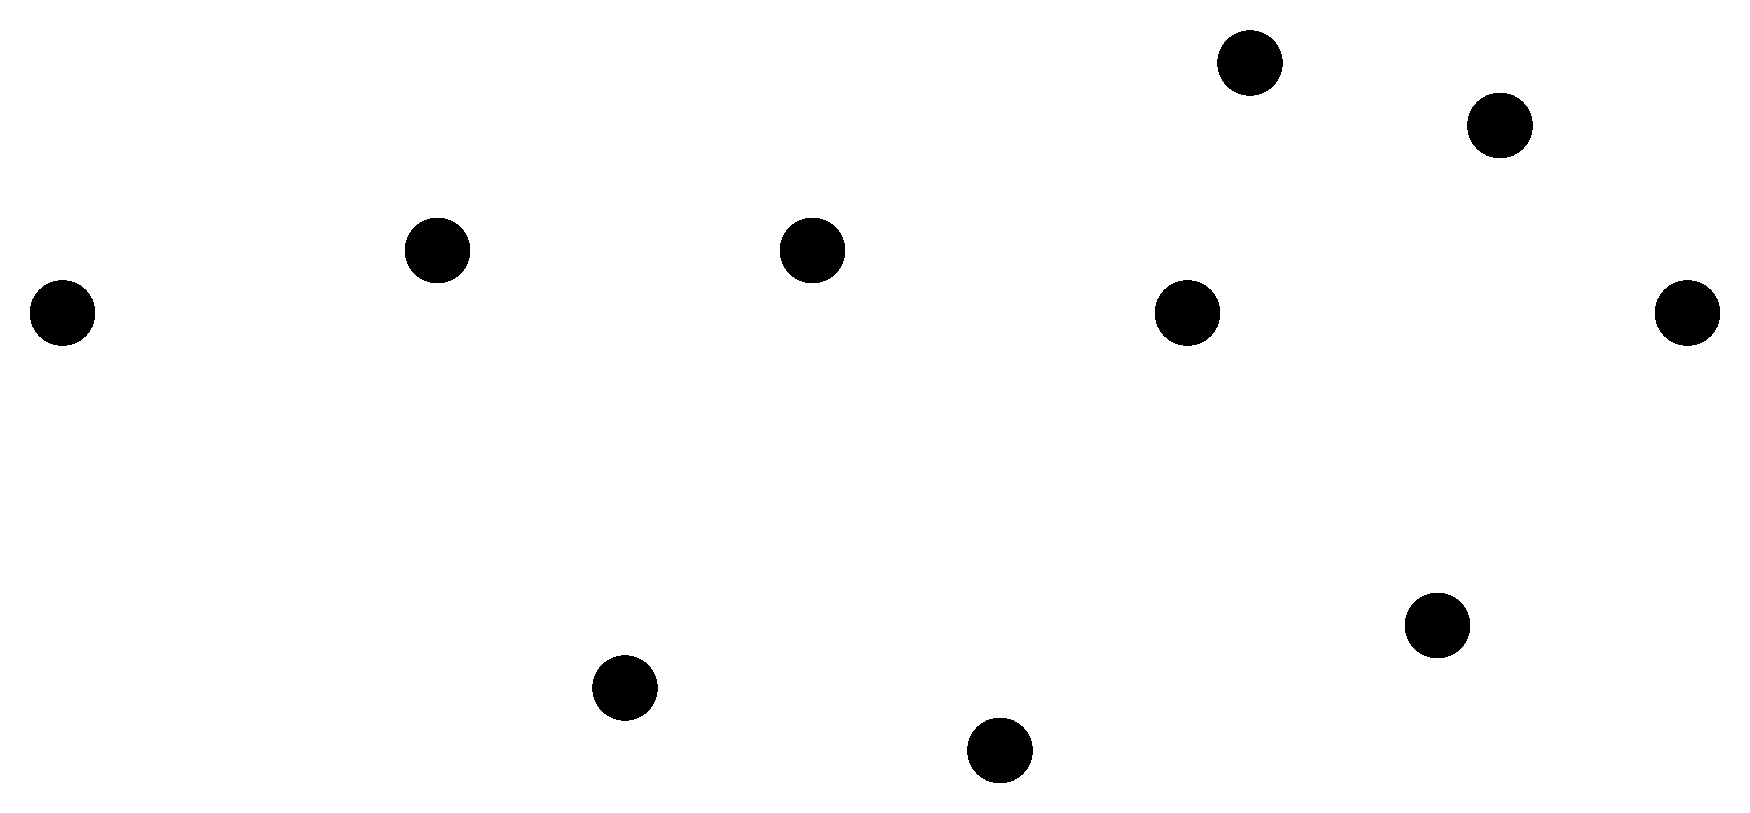
\includegraphics[width=5cm]{fig/graph_1_nodes.pdf}
\end{figure}%
%\end{frame}
\framebreak
%--------------------------------------------------------------------------%
%\begin{frame}
\frametitle{Attributed undirected graph}
Attributed undirected graph $G=(V,E,$
\begin{itemize}
\item set of nodes $V=\{v_i\}_{i=1}^{n}$
\item set of edges $E\subseteq\{\{u,v\}| u, v\in V\}$
\end{itemize}
\vspace{1.5cm}
\begin{figure}[b]
    \centering
    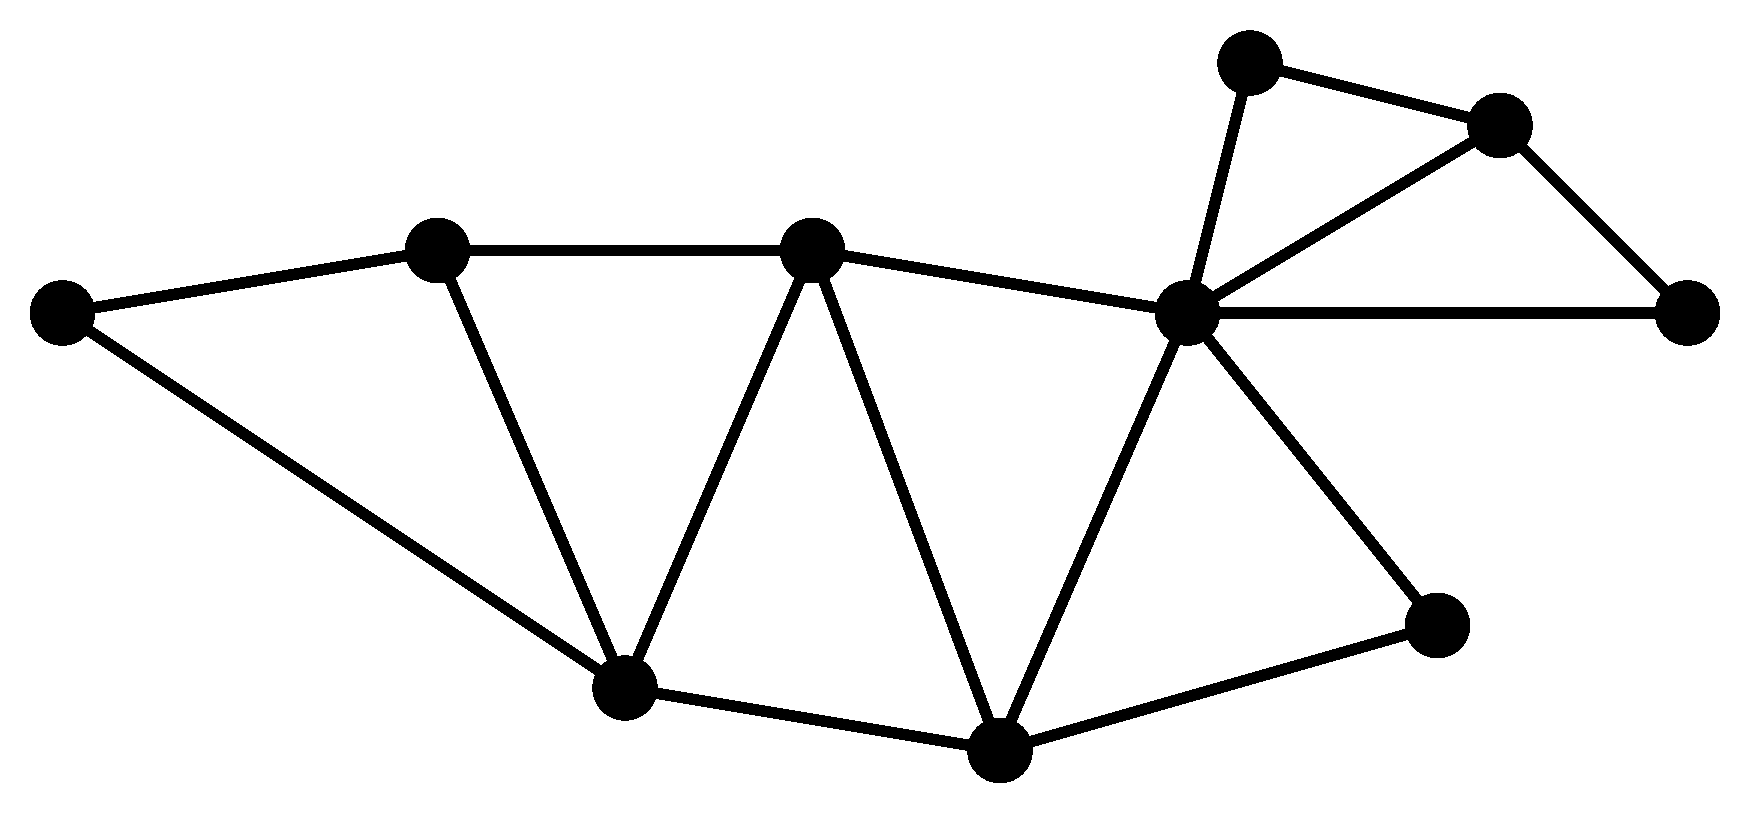
\includegraphics[width=5cm]{fig/graph_1.pdf}
\end{figure}%
\end{frame}
%--------------------------------------------------------------------------%
\begin{frame}
\frametitle{Attributed undirected graph}
Attributed undirected graph $G=(V,E,D)$
\begin{itemize}
\item set of nodes $V=\{v_i\}_{i=1}^{n}$
\item set of edges $E\subseteq\{\{u,v\}| u, v\in V\}$
\item node attributes $D=\{d_i\}_{i=1}^{n}$
\end{itemize}
\vspace{1cm}
\begin{figure}[b]
    \centering
    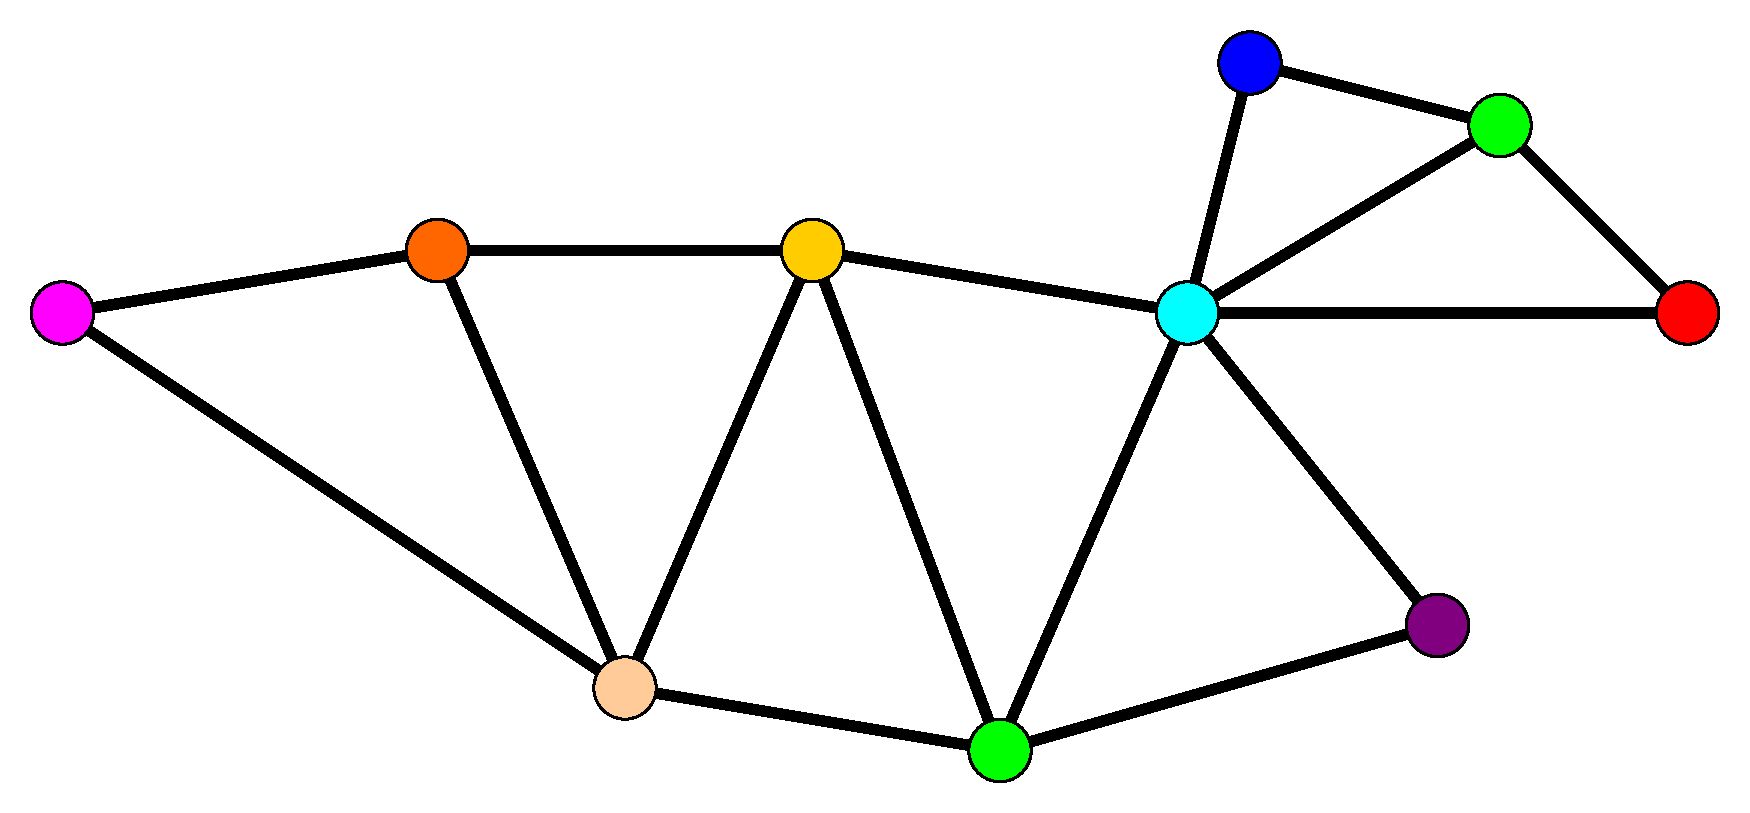
\includegraphics[width=5cm]{fig/at_graph_1.pdf}
\end{figure}%
\end{frame}
%--------------------------------------------------------------------------%
\begin{frame}
\frametitle{Graph matching}
Let us consider two undirected attributed graphs $G^I = (V^I, E^I, D^I)$ and $G^J = (V^J, E^J,D^J)$: % with $|V^I|=n_1$ and $|V^J|=n_2$:
\begin{figure}[h]
        \centering
        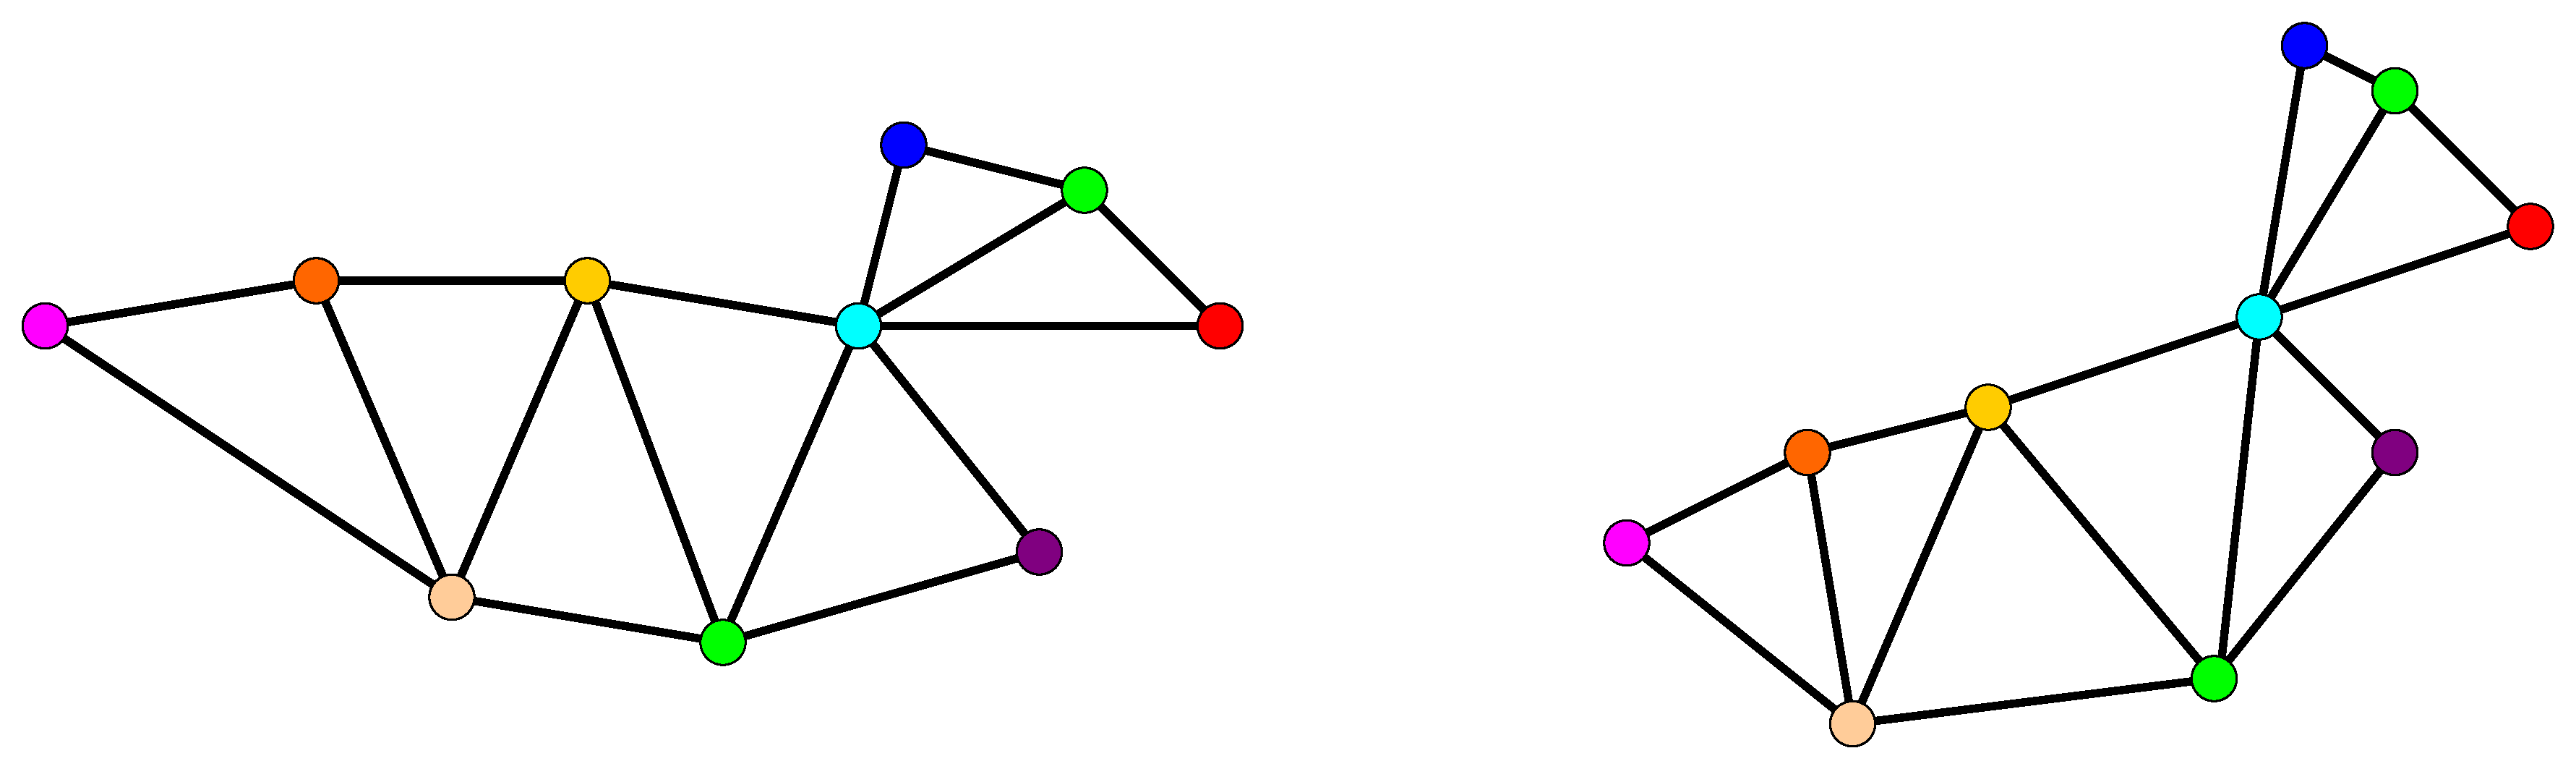
\includegraphics[width=6cm]{fig/graphs_12.pdf}
\end{figure}
%A matching function between $G^I$ and $G^J$ is a mapping $m:V^I\rightarrow V^J$ between the sets of nodes of two graphs.
\end{frame}
%\framebreak
%--------------------------------------------------------------------------%
\begin{frame}
\frametitle{Graph matching}
\begin{figure}[t]
        \centering
        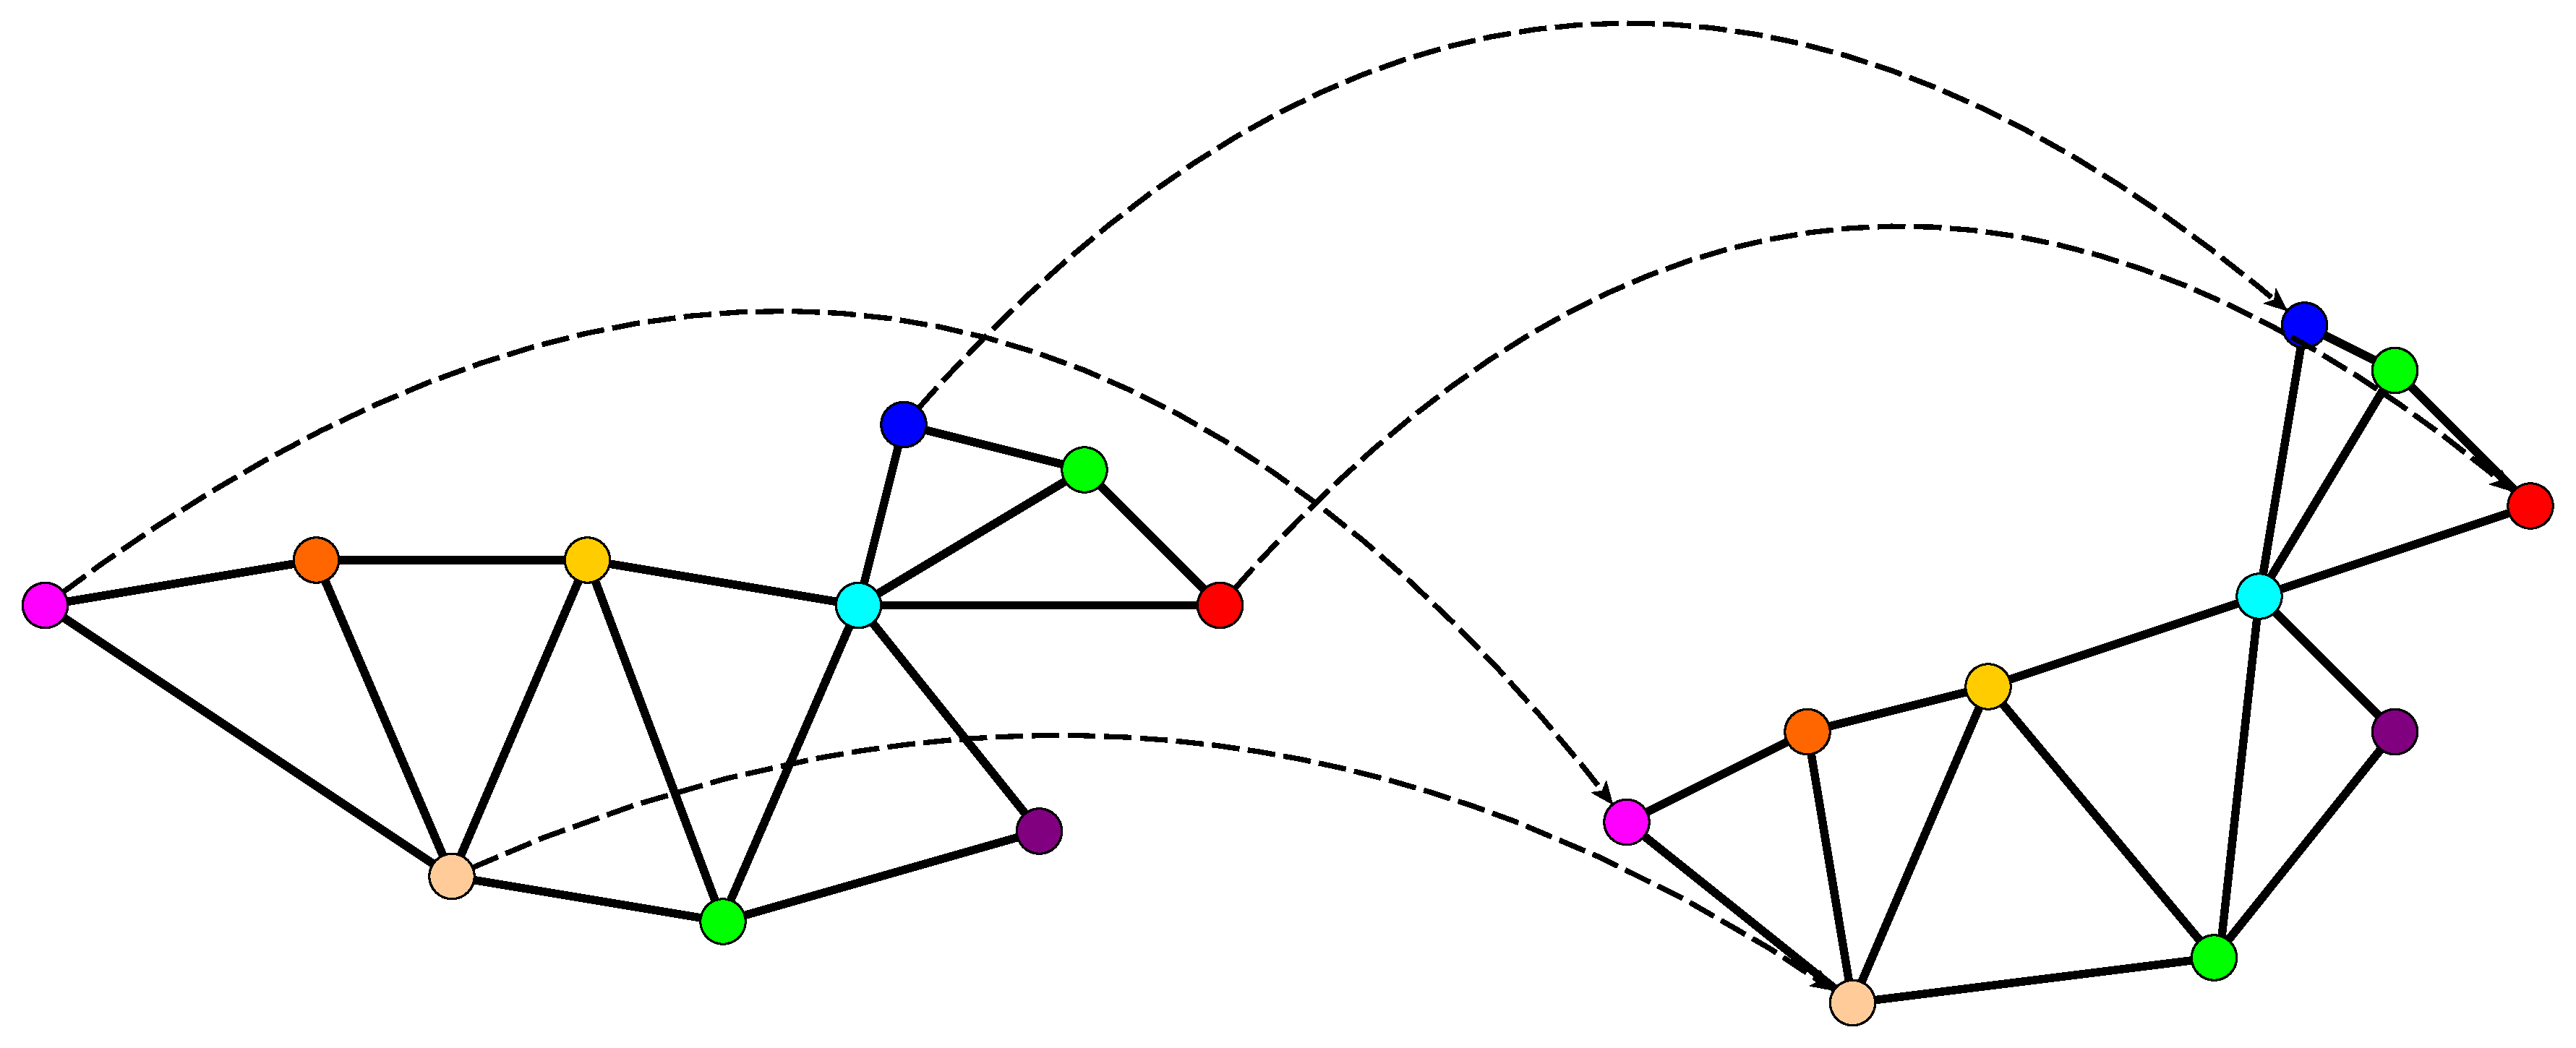
\includegraphics[width=5cm]{fig/matching_12.pdf}
\end{figure}
A matching function between $G^I$ and $G^J$ is a mapping %between the sets of nodes of two graphs:
\\
{\hspace{4cm}$m:V^I\rightarrow V^J$}
\visible<2>{\textcolor{red}{\hspace{2cm}not unique!}}
\visible<3->{
Define a function $S(G^I, G^J, m)$ to measure the quality of matching $m$ that fulfills some conditions\\
$\Rightarrow$ \textcolor{red}{Graph matching problem} between $G^I$ and $G^J$ 
\begin{equation*} \label{gGMP}
m = \argmax_{\hat{m}}S(G^I, G^J, \hat{m})
\end{equation*}
}
\end{frame}
%--------------------------------------------------------------------------%
\begin{frame}
\frametitle{Graph matching in computer vision}
\begin{figure}[t]
    \centering
    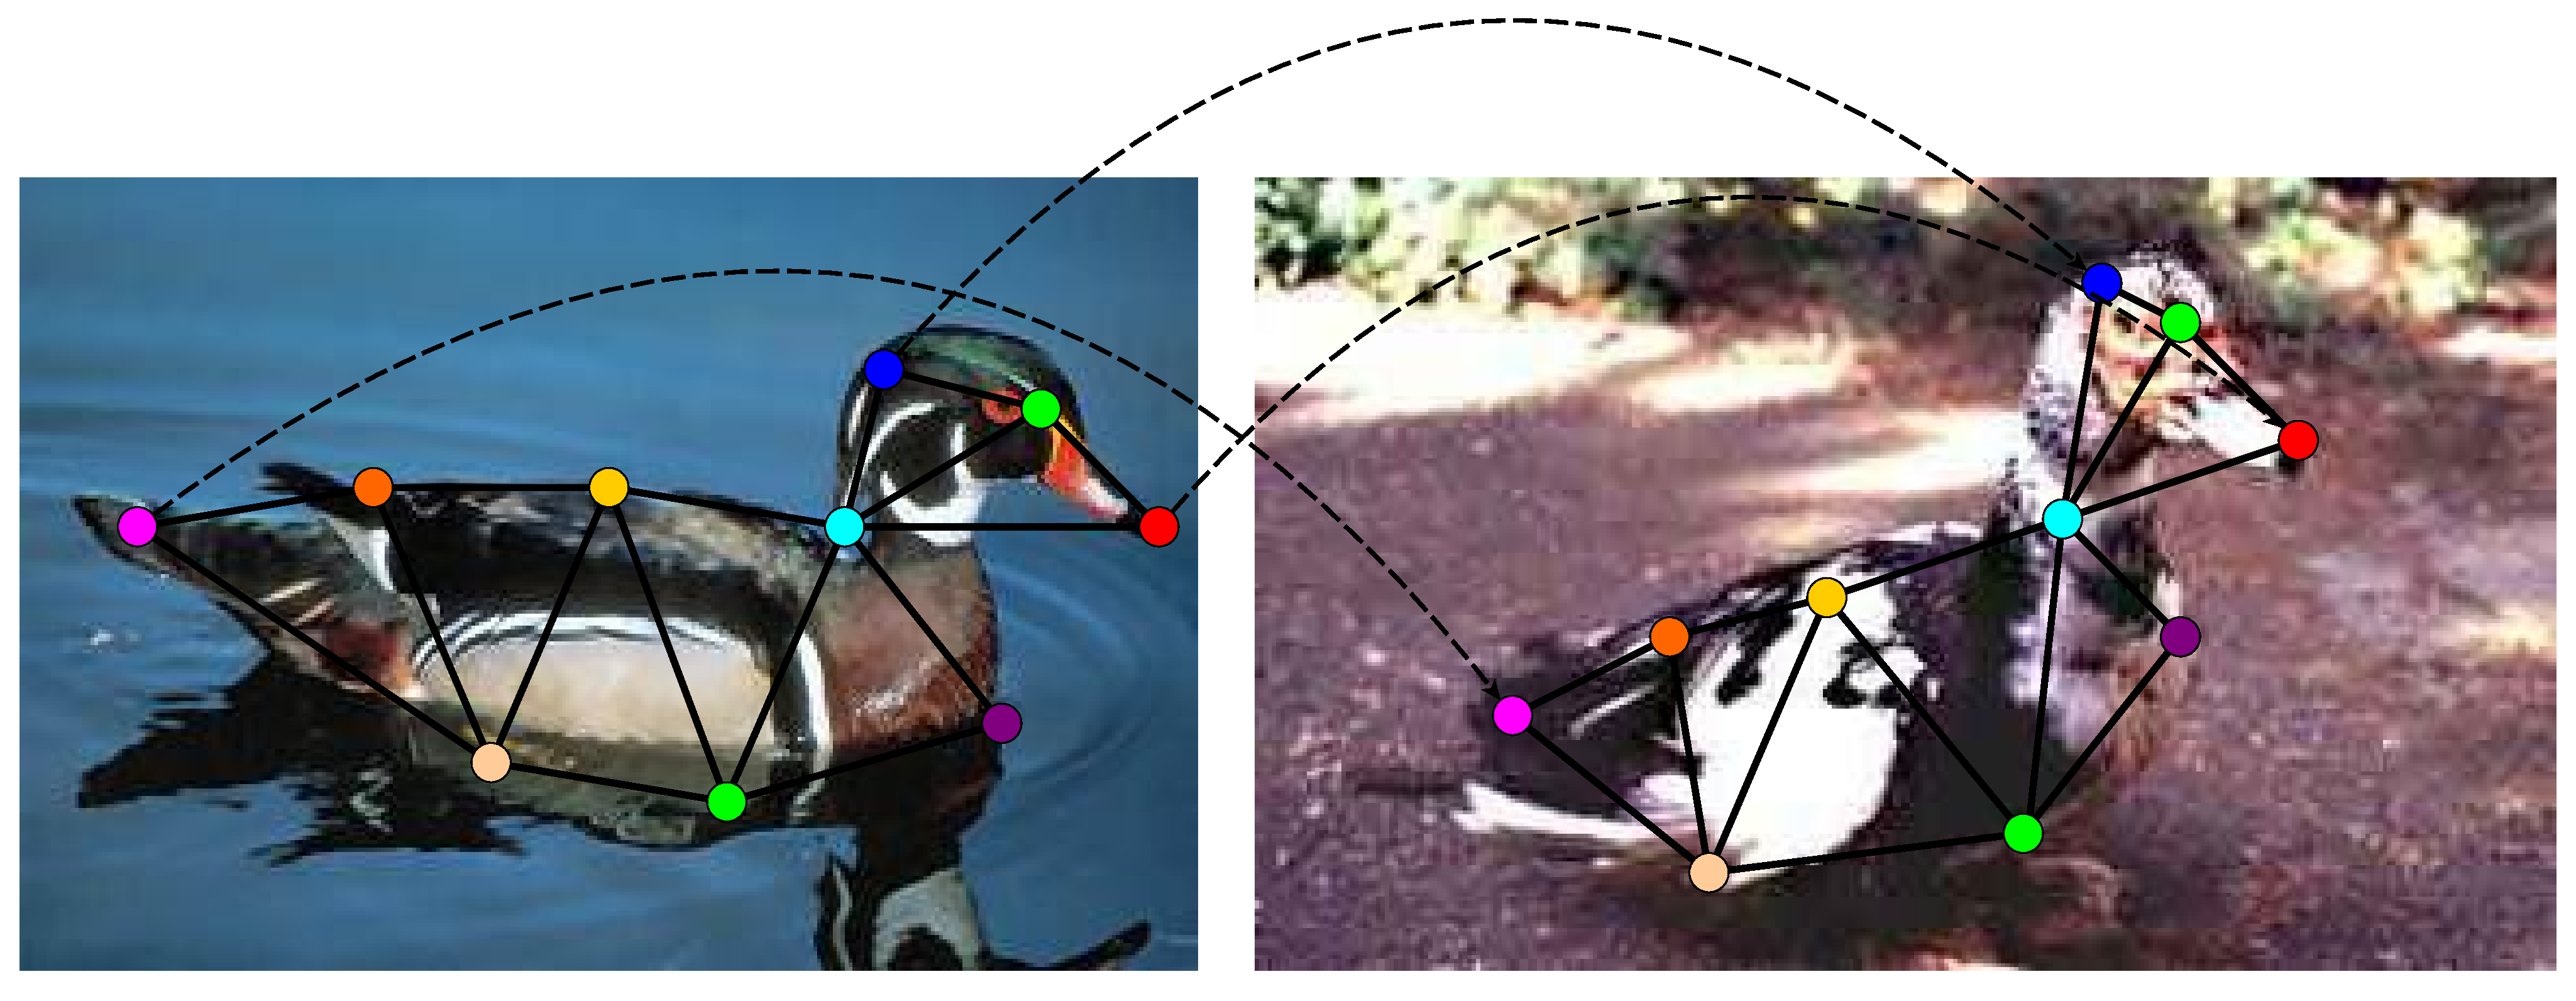
\includegraphics[width=5cm]{fig/ducks_12.pdf}
\end{figure}
\begin{itemize}
\item image matching
\item shape matching
\item object detection
\item object tracking
\item $\dots$
\end{itemize}
\end{frame}
%--------------------------------------------------------------------------%
\begin{frame}
\frametitle{Exact graph matching}
Edge preserving mapping $m$:\\
$\{v_i,v_{i^\prime}\}\in E^I\Rightarrow\{m(v),m(v_{i^\prime})\}\in E^J$ for all $v_i,v_{i^\prime}\in V^I$.


\begin{itemize}
\item mapping $m$ is bijective $\rightarrow$ graph isomorphism
\item mapping $m$ is injective $\rightarrow$ graph monomorphism
\item mapping $m$ is total\hspace{15pt} $\rightarrow$ graph homomorphism
\end{itemize}
\begin{figure}[h!]
    \centering
    \begin{subfigure}[b]{0.3\textwidth}
        \includegraphics[width=\textwidth]{fig/GI}
        \caption{Graph isomorphism}
        \label{fig:GI}
    \end{subfigure}
    ~
    \begin{subfigure}[b]{0.3\textwidth}
        \includegraphics[width=\textwidth]{fig/monomorphism}
        \caption{Graph monomorphism}
        \label{fig:monomorphism}
    \end{subfigure}
    ~
    \begin{subfigure}[b]{0.3\textwidth}
        \includegraphics[width=\textwidth]{fig/homomorphism}
        \caption{Graph homomorphism}
        \label{fig:homomorphism}
    \end{subfigure}
\end{figure}

\visible<2>{\textcolor{red}{\hspace{2cm}not unique!}}
\end{frame}

%--------------------------------------------------------------------------%
\begin{frame}
%\frametitle{Graph Matching}
Given two attributed graphs $\bar{G}^P=(\bar{V}^P, \bar{E}^P, \bar{A}^P)$ and $\bar{G}^Q=(\bar{V}^Q, \bar{E}^Q, \bar{A}^Q)$ with $n^P$ and $n^Q$ nodes respectively.

A result of graph matching is a subset of possible correspondences between those graphs, which can be represented in form of assignment matrix $X\in\{0,1\}^{n^P\times n^Q}$:
$$X_{ia} = \begin{cases} 1 & \mbox{node}\ v_i\in \bar{V}^P \mbox{matches}\ v_a \in \bar{V}^Q \\
						 0 & \mbox{otherwise} \\
			\end{cases}$$
General formulation:
$$x^* = \arg\max S(x)$$
$$ s.t. \begin{cases}
									x\in\{0,1\}^{n^Pn^Q} \\
								 \sum_{i=1}^{n^P}x_{ia}\le 1 \\
								 \sum_{a=1}^{n^Q}x_{ia}\le 1  \end{cases}$$
The objective function $S(x)$ measures the similarity between the graph attributes. 
\end{frame} 

%--------------------------------------------------------------------------%
%--------------------------------------------------------------------------%
\section{Solution techniques} 
\begin{frame}
\frametitle{Drei exemplarische Typen von Suchanfragen}
\begin{itemize}
\item spezielle: \hspace{50pt}
						\visible<2->{\textcolor{red}{Problem der Knappheit}} \\
	\glqq Does Netscape support the JDK 1.1 - code-signing API?\grqq
	\cite{Kleinberg}
	\begin{block}{}
	\item 
	breit angelegte: \hspace{30pt} 	
					\visible<3->{\textcolor{red}{Problem der Vielfältigkeit}} \\
	\glqq Find information about the Java programming language\grqq \cite{Kleinberg}
	\end{block}
	
	\item Suche nach ähnlichen Seiten\\
	\glqq Find pages similar to {\it java.sun.com}\grqq\cite{Kleinberg}
	
\end{itemize}
\end{frame}
%--------------------------------------------------------------------------%
\begin{frame}
\frametitle{Ranking}

\begin{itemize}
\item Man möchte die angesehensten Seiten (Authorities) aus der Menge aller zu der Anfrage relevanten Seiten finden
\item Mögliche Hindernisse:
	\begin{itemize}
	\item die höchst relevanten Seiten werden nicht unbedingt durch ein textbasiertes Ranking vorgezogen
	\item es kann sein,  dass die relevanten Seiten die Wörter aus der Suchanfrage gar nicht enthalten
	\end{itemize}
\end{itemize}
\end{frame}
%--------------------------------------------------------------------------%
\begin{frame}[allowframebreaks]

\begin{block}{Annahme}
Die Relevanz zwischen zwei Seiten wurde vom Ersteller des Links zwischen diesen Seiten geprüft
\end{block}

Stimmt im Allgemeinen nicht (z.B. Navigationslinks, Werbung)
\vspace{10pt}

Aber unter dieser Annahme reicht es, nur die Linkstruktur des WWW zu betrachten, um die Autorität einer Seite im Bezug auf eine andere zu bestimmen

\frametitle{Authorities und Hubs}

\framebreak

\begin{block}{Authorities (Autoritätsseiten)}
Relevante Seiten, auf die viele weitere relevante Seiten zeigen
\end{block}


\begin{block}{Hubs}
Seiten, die auf viele Authorities zeigen
\end{block}

\end{frame}
%--------------------------------------------------------------------------%
%--------------------------------------------------------------------------%
\section{2LevelGM} 


%--------------------------------------------------------------------------%
%--------------------------------------------------------------------------%
\section{Evaluation} 

%--------------------------------------------------------------------------%
%--------------------------------------------------------------------------%
\section*{The End}
\begin{frame}{The end}
\centering
\LARGE
\color{red}
Thank you for your attention!
%\nocite{Kleinberg}
%\nocite{ZheZhao2}
%\nocite{CIS}
%\nocite{HITS_Lecture4_Cornell}
%\nocite{BeamerTheme} 
\nocite{Cho_LearningG}
\end{frame}
%--------------------------------------------------------------------------%
\begin{frame}
\centering
\begin{figure}
	\includegraphics{who.png}
\end{figure}
\end{frame}
%--------------------------------------------------------------------------%
\begin{frame}[allowframebreaks]
	\frametitle{References}
	\bibliographystyle{plain}
	\bibliography{bibliographie}
\end{frame} 

\end{document}
%--------------------------------------------------------------------------%
%--------------------------------------------------------------------------%
%--------------------------------------------------------------------------%
